\documentclass[main]{subfiles}

\begin{document}
    \Date{08.10.19}

    \begin{Task}[стереографическая проекция]
      \[f: S^2 -\{(0,0,1)\} \ra \R^2,\q (x,y,z) \mapsto \Br{\dfrac{x}{1-z},\ \dfrac{y}{1-z}}\]
      \[\text{где } S^2=\{(x,y,z) \in \R^3 \mid x^2 + y^2 + z^2 = 1\}\]
      \begin{enumerate}
        \item Найдите $f^{-1}=g \q \R^2 \ra S^2 - \{N\}$ (полюс)
        \item Доказать, что g сохраняет углы
        \item Найдите $\RNumb{1}(F)$ (п.ф.ф.) g
      \end{enumerate}
    \end{Task}

    \begin{Sol} \
      \begin{figure}[H]
          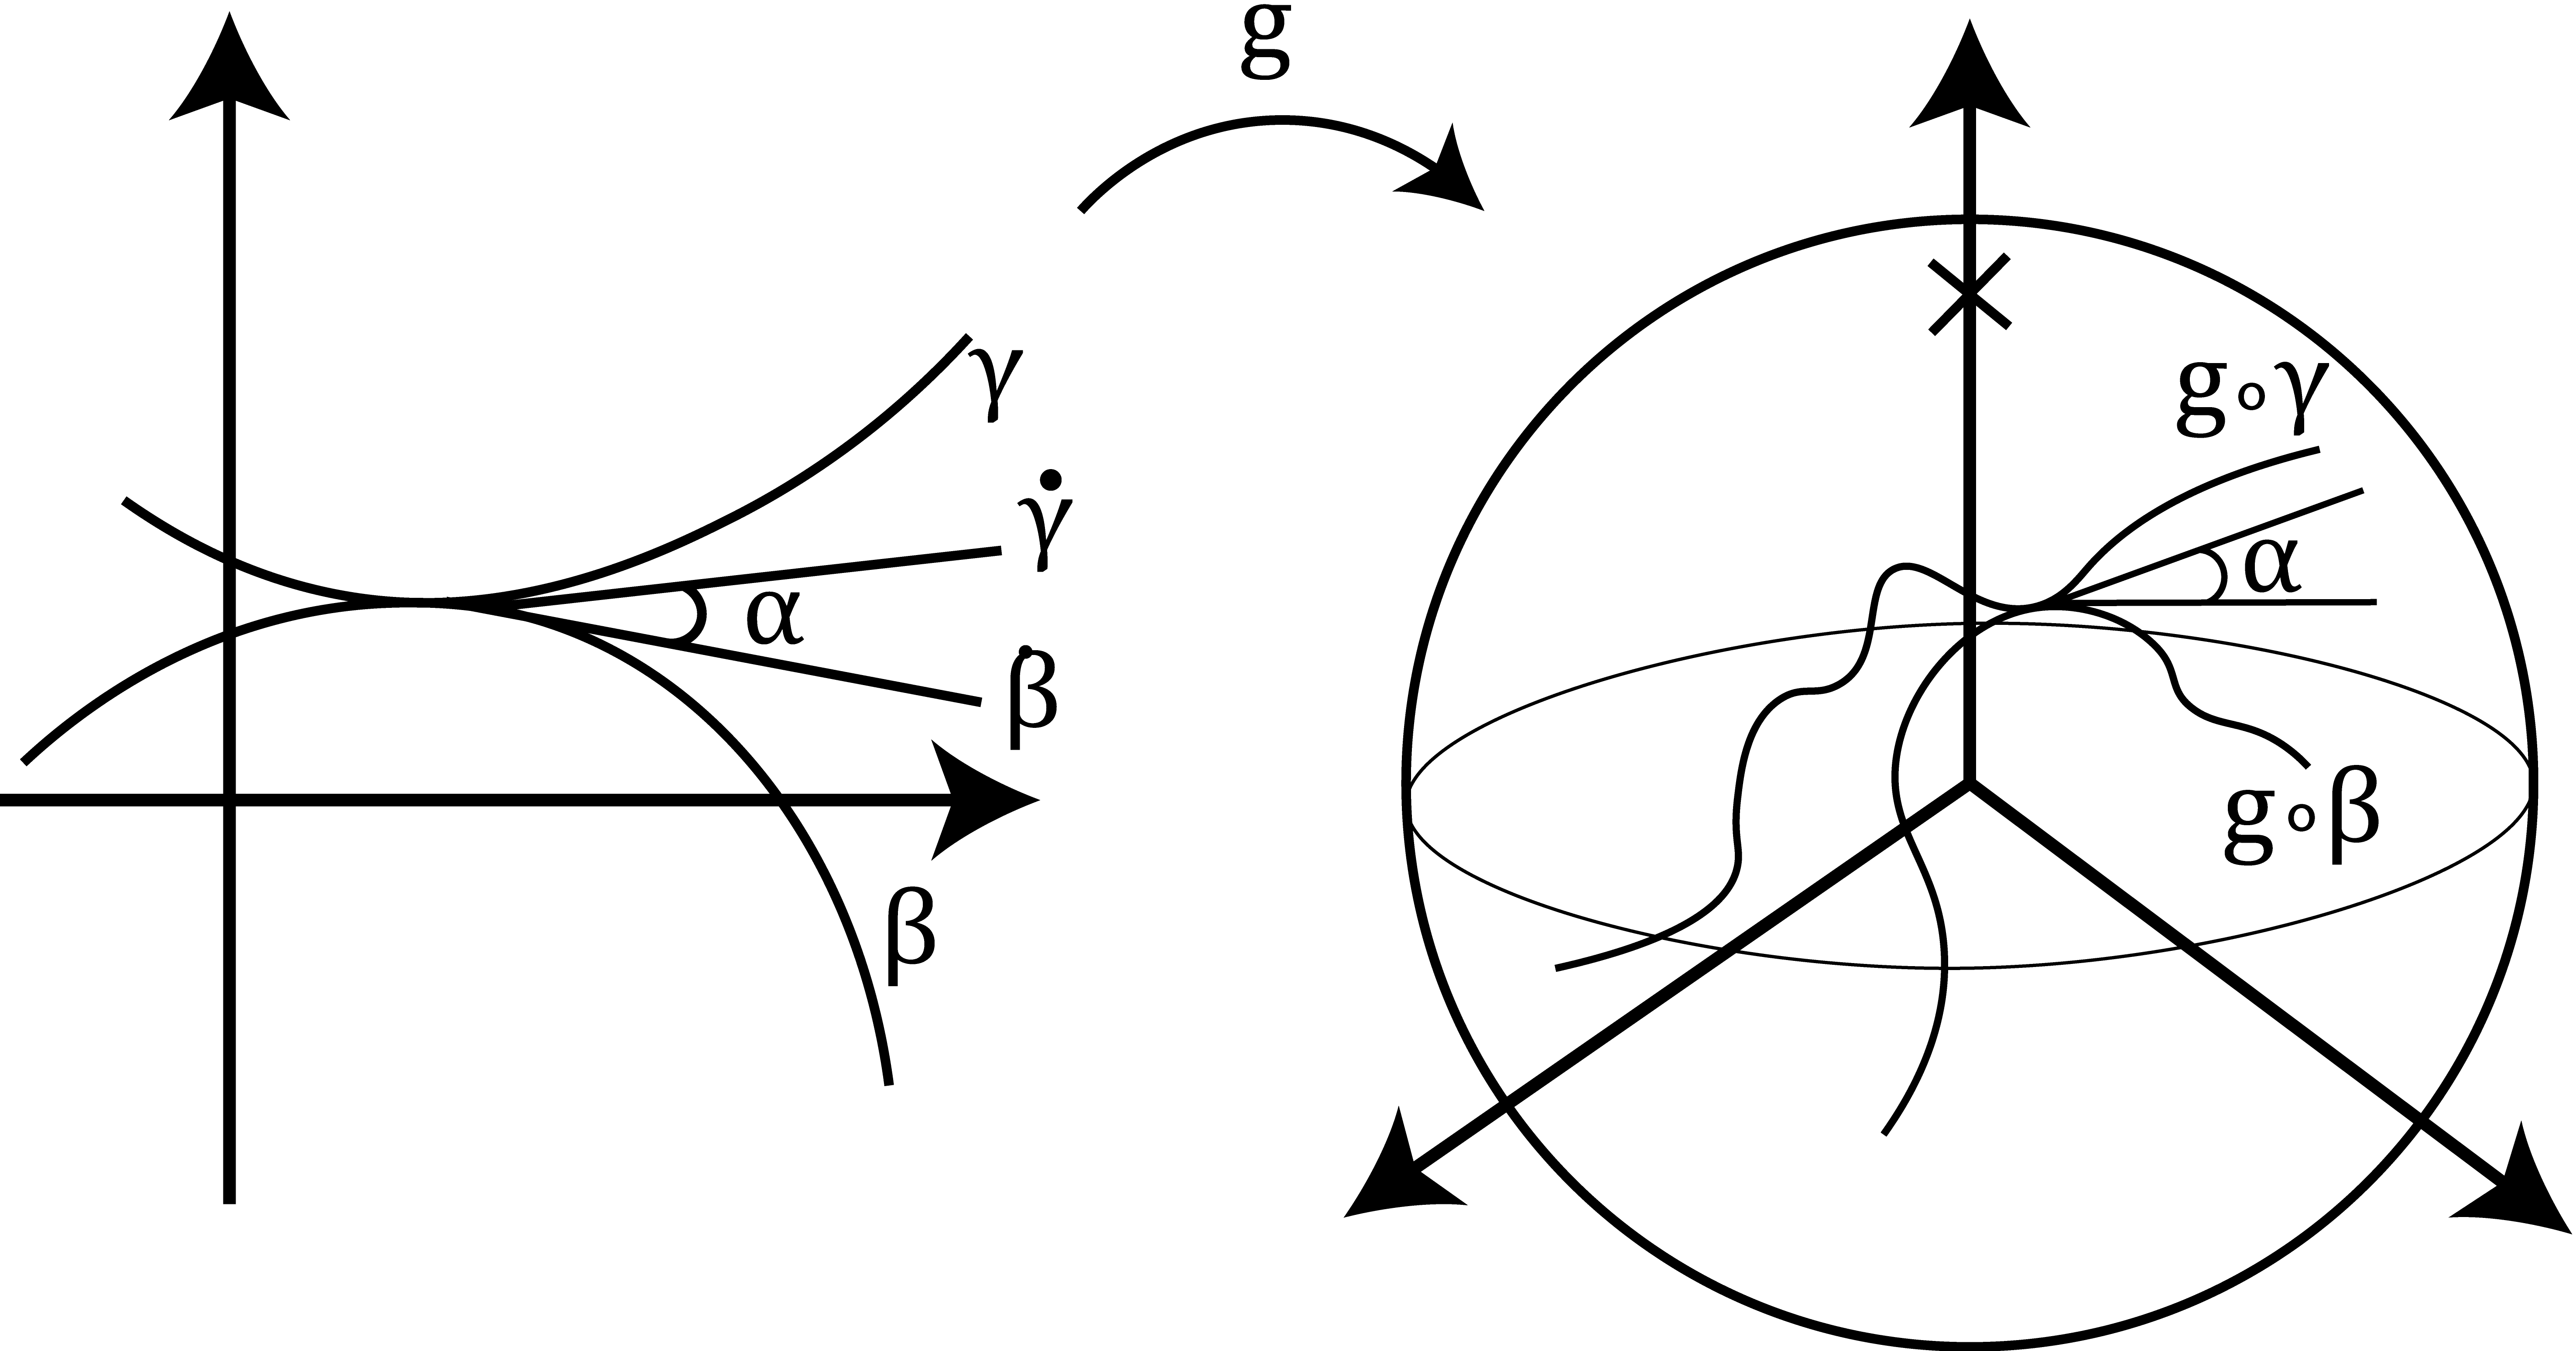
\includegraphics[width=9cm]{pics/7_1}
          \centering
      \end{figure}
      \begin{enumerate}
        \item Надо найти g: $f \circ g = \id$ и $g \circ f = \id$
        \[a = \dfrac{x}{1-z},\q b = \dfrac{y}{1-z},\q x^2 + y^2 + z^2 = 1\]
        Найдем из уравнений $x,y,z$:
        \[z = \dfrac{a^2 + b^2 - 1}{a^2 + b^2 + 1},\q
        x = \dfrac{2a}{a^2 + b^2 + 1},\q
        y=\dfrac{2b}{a^2 + b^2 + 1}\]
        \item Вспомним, что
        \[\cos (\alpha) = \dfrac{<\dot{\gamma},\ \dot{\beta}>}{\abs{\dot{\gamma}} \abs{\dot{\beta}}},\qq
        \cos (\theta) = \dfrac{<\dot{\w{\gamma}},\ \dot{\w{\beta}}>}{\abs{\dot{\w{\gamma}}} \abs{\dot{\w{\beta}}}}\]
        \[\w{\gamma} = g \circ \gamma\q \w{\beta} = g \circ \beta\]
        \[\w{\gamma} = \Br{
          \dfrac{2 \gamma_1}{{\gamma_1}^2 + {\gamma_2}^2 + 1},\
          \dfrac{2 \gamma_2}{{\gamma_1}^2 + {\gamma_2}^2 + 1},\
          \dfrac{{\gamma_1}^2 + {\gamma_2}^2 - 1}{{\gamma_1}^2 + {\gamma_2}^2 + 1}
        }\]
        Аналогично другие. Можно было бы посчитать всё и подставить
        \[\dfrac{d}{dt} \w{\gamma} = \dfrac{\d g}{\d a} \dot{\gamma}_1 + \dfrac{\d g}{\d b} \dot{\gamma}_2\]
        Обозначим $\bigstar = a^2 + b^2 + 1$
        \[\dfrac{\d g}{\d a} = \Br{
          \dfrac{2\bigstar-4a^2}{\bigstar^2},\
          \dfrac{2\bigstar-4b^2}{\bigstar^2},\
          \dfrac{4b}{\bigstar^2}
        }\]
        \[\RNumb{1}(F) = \begin{pmatrix}
          \os{=\rho}{<\dfrac{\d g}{\d a},\ \dfrac{\d g}{\d a}>} & \os{=0}{<\dfrac{\d g}{\d b},\ \dfrac{\d g}{\d a}>}\\ \\
          \us{=0}{<\dfrac{\d g}{\d a},\ \dfrac{\d g}{\d b}>} & \us{=\rho}{<\dfrac{\d g}{\d b},\ \dfrac{\d g}{\d \mathbf{}}>}
        \end{pmatrix} = \begin{pmatrix}
          \rho & 0\\
          0 & \rho
        \end{pmatrix}\]
        То есть на самом деле:
        \[\cos (\theta) = \dfrac{<\dot{\w{\gamma}},\ \dot{\w{\beta}}>}{|\w{\gamma}| |\w{\beta}|} =
        \dfrac{<\dot{\gamma},\ \RNumb{1}\dot{\beta}>}
          {\sqrt{<\dot{\gamma},\ \RNumb{1} \dot{\gamma}>} \sqrt{<\dot{\beta},\ \RNumb{1} \dot{\beta}>}}\]
        \[\w{\gamma} =
        <\dfrac{\d g}{\d a} \dot{\gamma_1} + \dfrac{\d g}{\d b} \dot{\gamma_2},\
        \dfrac{\d g}{\d a} \dot{\gamma_1} + \dfrac{\d g}{\d b} \dot{\gamma_2}>\]
        \[<\w{\dot{\gamma}},\ \w{\dot{\gamma}}> =
        <\dfrac{\d g}{\d a},\ \dfrac{\d g}{\d a}> \dot{\gamma}_1^2 +
        2<\dfrac{\d g}{\d a},\ \dfrac{\d g}{\d b}> \dot{\gamma}_1 \dot{\gamma}_2 +
        <\dfrac{\d g}{\d b},\ \dfrac{\d g}{\d b}> \dot{\gamma}_2^2\]
        \[ = <\begin{pmatrix}
          \dot{\gamma}_1 \\
          \dot{\gamma}_2
      \end{pmatrix},\ \RNumb{1}> <\begin{pmatrix}
          \dot{\gamma}_1 \\
          \dot{\gamma}_2
        \end{pmatrix}\]
        \[\dfrac{\rho <\dot{\gamma},\ \dot{\beta}>}{\sqrt{\rho} |\dot{\gamma}| \sqrt{\rho} |\dot{\beta}|}
        = \dfrac{\rho<\dot{\gamma},\ \dot{\beta}>}{\rho |\dot{\gamma}| |\dot{\beta}|}
        = \dfrac{<\dot{\gamma},\ \dot{\beta}>}{|\dot{\gamma}| |\dot{\beta}|}
        = \cos \alpha\]
        \item см. выше
      \end{enumerate}
    \end{Sol}
\end{document}
